
\subsection{Vista de Persona}
\label{sub:vista_persona}
Se creó una vista mediante la cual se pueda acceder a la información de cada persona y a la lista de actividades en las que se encuentra involucrada. Su
implementación se basó en la iteración de la colección de actividades  de la persona y la generación de html mediante \textbf{Twig}\@.
Como último paso se agregó estilo mediante \textbf{CSS} y una simple animación en \textbf{Javascript}.


\subsubsection{Estilo}%
\label{ssub:estilo}

Se utilizó una distribución de elementos utilizando \textit{grid}, una característica de \textbf{CSS} que permite acomodar elementos en una grilla.




% TODO   franco continuar vie 01 nov 2019 20:37:16 -03

\begin{figure}[h]
    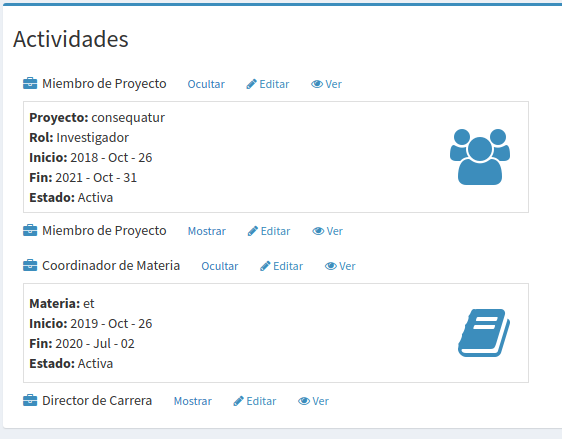
\includegraphics[width=1\linewidth]{image/vista_persona.png}
    \caption{Listado de actividades.\newline \textbf{Fuente:} Elaboración propia, captura de pantalla de aplicación web.}
    \label{fig:image/vista_persona}
\end{figure}


\begin{figure}[h]
    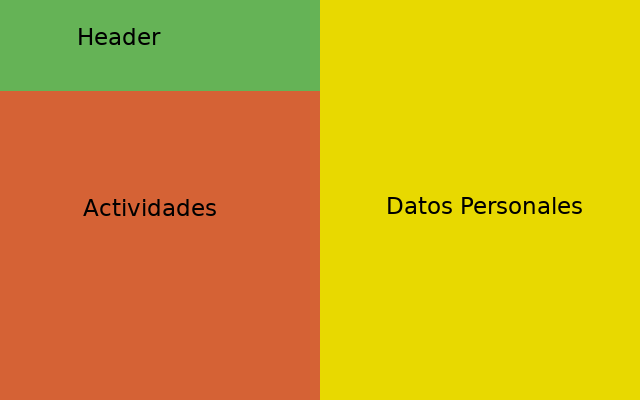
\includegraphics[width=1\linewidth]{image/grid.png}
    \caption{Distribución de columnas y filas.\newline \textbf{Fuente:} Elaboración propia.}
    \label{fig:image/grid}
\end{figure}
